\documentclass[11pt]{article}

\usepackage[margin=1in]{geometry}
\usepackage[utf8]{inputenc}
\usepackage[T1]{fontenc}
\usepackage{times}
\usepackage{microtype}
\usepackage{amsmath,amssymb,amsthm}
\usepackage{booktabs}
\usepackage{caption}
\captionsetup[table]{skip=6pt}
\usepackage{graphicx}
\usepackage{xcolor}
\usepackage[numbers,sort&compress]{natbib}
\usepackage[colorlinks=true,linkcolor=blue!60!black,citecolor=blue!60!black,urlcolor=blue!60!black]{hyperref}
\usepackage[capitalize,noabbrev]{cleveref}

\newcommand{\R}{\mathbb{R}}
\newcommand{\vpgdmin}{0.84}
\newcommand{\vpgdmax}{0.93}
\newcommand{\vjgdmin}{0.54}
\newcommand{\vjgdmax}{0.80}
\newcommand{\cleanmin}{0.96}
\newcommand{\cleanmax}{1.07}
\newcommand{\gpmcleanmax}{5.8}
\newcommand{\gdgpmSfourmin}{0.10}
\newcommand{\gdgpmSfourmax}{0.11}
\newcommand{\mainDelta}{-0.91}
\newcommand{\mainDeltaLo}{-1.89}
\newcommand{\mainDeltaHi}{0.06}
\newcommand{\mainVPGD}{-1.35}
\newcommand{\mainVPGDLo}{-2.70}
\newcommand{\mainVPGDHi}{-0.01}
\newcommand{\maxDeltaHi}{7.12}
\newcommand{\bestDelta}{5.29}
\newcommand{\nkilled}{7}
\newcommand{\nconfigs}{8}
\newcommand{\nseeds}{16}
\newcommand{\runtime}{7}
\newcommand{\jointAmin}{14}
\newcommand{\hlAgpm}{0.167}
\newcommand{\hlAjoint}{0.122}
\newcommand{\hlBvpSfourmax}{0.041}
\newcommand{\cvpexact}{0.56}
\newcommand{\swmin}{0.31}
\newcommand{\swmax}{4.66}
\newcommand{\swlomin}{0.00}
\newcommand{\swwmin}{5.7}
\newcommand{\swwmax}{24.1}
\newcommand{\swAmin}{1.00}
\newcommand{\hardDelta}{5.29}
\newcommand{\hardDeltaLo}{3.46}
\newcommand{\hardDeltaHi}{7.12}
\newcommand{\owmAmin}{55}


\title{\textbf{Dirty-Paper Writes Make Old Weights Free\\but Do Not Beat Projection}}
\author{Manoj Bajaj}
\date{}
\hypersetup{pdftitle={Dirty-Paper Writes Make Old Weights Free but Do Not Beat Projection},pdfauthor={Manoj Bajaj}}

\begin{document}
\maketitle

\begin{abstract}
Costa's dirty-paper theorem says interference known to the encoder costs no capacity.
Read as a continual-learning rule, a new task could be precoded against the known old weights instead of being projected away from them.
We test this in the one setting where the premise holds exactly: a ReLU network whose readout is decoded modulo 8, written by lattice precoding.
Known old weights do become free: across \nconfigs{} interference levels and \nseeds{} seeds, the minimum-norm precoded write costs \cleanmin--\cleanmax{} times an interference-free write, whereas plain gradient projection memory (GPM) pays up to \gpmcleanmax{} times.
But the pre-registered test, new-task accuracy at equal update norm with old-task accuracy held to GPM's, fails in \nkilled{} of \nconfigs{} configurations.
Projected gradient descent on the same periodic loss captures most of the saving, and old-task accuracy cannot improve on GPM's 100\%.
A joint precoder that shifts old outputs by whole periods needs 20--46\% less norm for an exact write, yet drops old-task accuracy to \jointAmin\% when the budget falls short.
Dirty-paper coding therefore offers write norm, not retention.
\end{abstract}

\section{Introduction}
\label{sec:intro}

Projection methods protect an old task by writing the new one only in directions the old task does not use~\citep{zeng2019owm,farajtabar2020ogd,saha2021gpm}.
They treat the old weights as something to avoid.
Information theory suggests a different stance.
When a channel adds interference that the transmitter knows in advance, Costa showed that the capacity equals that of a channel with no interference at all~\citep{costa1983,gelfand1980}: the transmitter precodes around the interference instead of cancelling it.
A continual learner knows its old weights exactly, so the analogy proposes \emph{dirty-paper writes}: precode the new task's update against the old weights, and old knowledge should cost no write capacity.

The theorem needs more than known interference; it needs a decoder that folds the signal modulo a lattice~\citep{erez2005lattice}.
Ordinary readouts are not periodic, and for them the precoding coset collapses to a single point and the dirty-paper write is GPM (\cref{sec:scope}).
We therefore build the most favorable case: a two-layer ReLU network whose readout labels are residues modulo \(M=8\), so that every lattice precoder from communications applies verbatim.
If dirty-paper writes cannot beat projection here, they cannot beat it with a standard decoder.

The premise holds (\cref{tab:main}): the best precoded write's norm is within 7\% of an interference-free write's at every interference level, while GPM pays up to \gpmcleanmax{} times more when the old outputs span several periods.
The proposed gain does not follow.
\Cref{fig:budget} shows why at the main configuration: the same coset freedom is available to GPM by descending the periodic loss, and that baseline reaches the same new-task accuracy at every norm.
The joint precoder that moves old outputs by whole periods is the only arm that writes with markedly less norm, and it pays for the saving with old-task accuracy below its threshold.
Our contributions are:
\begin{itemize}
  \item a matched test of dirty-paper writes against GPM, OWM and GPM with modular descent at 15 equal update norms, \nconfigs{} configurations and \nseeds{} seeds, with a pre-registered kill bar (\cref{sec:method});
  \item a negative result: the dirty-paper arms do not beat projection on old-task accuracy anywhere and fail the new-task bar in \nkilled{} of \nconfigs{} configurations (\cref{sec:results});
  \item the exact place where the analogy breaks: Costa's saving survives, but it is a saving in write norm, which a cheaper modular descent mostly recovers and which the one arm that keeps it converts into a retention cliff (\cref{sec:scope}).
\end{itemize}

\begin{figure}[!t]
  \centering
  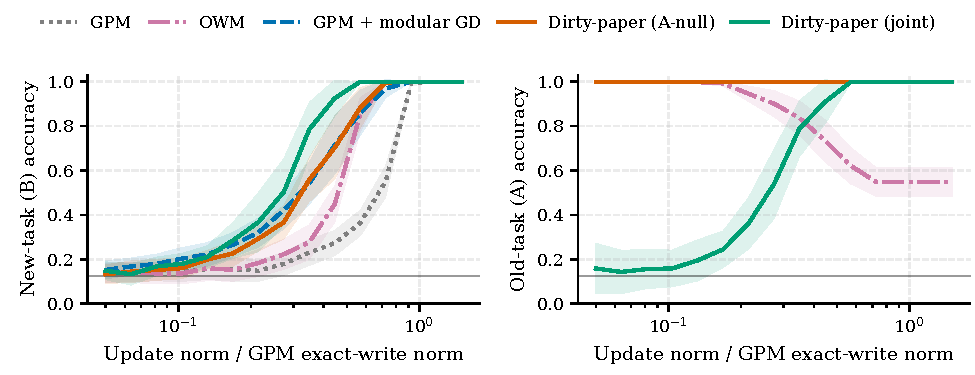
\includegraphics[width=\textwidth]{budget.pdf}
  \caption{\textbf{At equal update norm, dirty-paper writes do not beat projection.}
  Main configuration (\(\vartheta=30^\circ\), \(S=0\)); the horizontal axis is the update norm as a fraction of GPM's exact-write norm.
  Left: new-task accuracy. The A-null dirty-paper write tracks GPM with modular descent at every norm. The joint write learns earlier.
  Right: old-task accuracy. Every A-null arm keeps 100\%, so no write can beat GPM on the primary metric. The joint write and OWM lose old items when the norm is short.
  Lines are means over \nseeds{} seeds, bands 95\% Student-\(t\) intervals, and the gray line is chance (\(1/8\)).}
  \label{fig:budget}
\end{figure}

\section{A write channel where Costa's premise holds}
\label{sec:method}

\subsection{Network, tasks and decoder}

The network is a two-layer ReLU MLP with a frozen hidden layer and a scalar readout \(w\in\R^{h}\):
\(f_w(x)=w^\top\phi(x)\), \(\phi(x)=\sqrt{2/h}\,\max(Ux+c,0)\), with \(x\in\R^{16}\), \(h=64\), \(U_{ij}\sim\mathcal N(0,1/16)\) and \(c_i\sim\mathcal N(0,1/4)\).
Each item carries a residue label \(t\in\{0,\dots,M-1\}\) with \(M=8\), and is correct when \(f_w(x)\) rounds to \(t\) modulo \(M\):
\begin{equation}
  \mathrm{correct}(x,t)=\mathbf{1}\big[\,|\mathrm{wrap}(f_w(x)-t)|<\tfrac12\,\big],\qquad \mathrm{wrap}(u)=u-M\,\mathrm{round}(u/M).
  \label{eq:decoder}
\end{equation}
Chance is \(1/M=12.5\%\).
This modulo decoder is the assumption that makes dirty-paper coding possible (\cref{sec:scope}); everything else is a standard readout write.

Old task \(A\) has \(N_A=24\) Gaussian inputs with features \(\Phi_A\in\R^{h\times N_A}\) and uniform labels \(t_A\).
The old weights \(w_0\) are the minimum-norm interpolant of \(y_A=t_A+ML\), where \(L\) is uniform on \(\{-S,\dots,S\}\).
With \(S=0\) the old outputs sit in \([0,M)\); with \(S=4\) they are spread over five periods, as they would be after unconstrained training on a periodic loss.
New task \(B\) has \(N_B=16\) inputs, each at angle \(\vartheta\in\{15^\circ,30^\circ,60^\circ,90^\circ\}\) from a distinct \(A\) input, so smaller \(\vartheta\) means stronger interference.
The writer knows \(w_0\), so it knows the interference \(s_B=\Phi_B^\top w_0\) that the old weights add to every \(B\) output.

\subsection{Seven writes}

Every arm writes \(\Delta=Fa\) for a feature map \(F\) and asks for a change \(z\) of the outputs it controls; the exact write is the minimum-norm \(\Delta\) realizing \(z\).
Let \(P=I-\Phi_A(\Phi_A^\top\Phi_A)^{-1}\Phi_A^\top\) project onto the complement of \(A\)'s features, \(G=\Phi_B^\top P\Phi_B\), and \(r=t_B-s_B\).
\begin{itemize}
  \item \textbf{FT}: \(F=\Phi_B\), \(z=r\). No protection; a lower bound on norm and on retention.
  \item \textbf{GPM}~\citep{saha2021gpm}: \(F=P\Phi_B\), \(z=r\). Hard projection; \(A\)'s outputs do not move.
  \item \textbf{OWM}~\citep{zeng2019owm}: \(F=P_\alpha\Phi_B\), \(z=r\), with \(P_\alpha=I-\Phi_A(\Phi_A^\top\Phi_A+\alpha I)^{-1}\Phi_A^\top\) and \(\alpha=0.01\,\mathrm{tr}(\Phi_A^\top\Phi_A)/N_A\). Soft projection; \(A\) may move.
  \item \textbf{GPM + modular GD}: \(F=P\Phi_B\), trained by gradient descent on the periodic loss \(\tfrac{M^2}{4\pi^2}(1-\cos\tfrac{2\pi e}{M})\) of the residual \(e=s_B+G a-t_B\), for 60{,}000 steps at rate \(1/\lambda_{\max}(G)\).
  This is GPM given the same decoder knowledge as the dirty-paper arms, and is the strongest matched baseline.
  \item \textbf{Dirty-paper, THP}: \(F=P\Phi_B\), \(z=\mathrm{wrap}(r)\) coordinatewise: Tomlinson--Harashima precoding~\citep{tomlinson1971,harashima1972}.
  \item \textbf{Dirty-paper, A-null (VP)}: \(F=P\Phi_B\) and \(z\) the member of the coset \(r+M\mathbb Z^{N_B}\) of least write cost \(z^\top G^{-1}z\), i.e.\ vector-perturbation precoding~\citep{hochwald2005vp}.
  This is exactly the minimum-norm \(A\)-null write that decodes all of \(B\).
  \item \textbf{Dirty-paper, joint}: \(F=[\Phi_A,\Phi_B]\), with \(A\)'s outputs allowed to move by whole periods: \(z\in M\mathbb Z^{N_A}\times(r+M\mathbb Z^{N_B})\), minimizing \(z^\top K^{-1}z\) with \(K=F^\top F\).
  The new task is written \emph{around} the old one instead of beside it, which is the card's literal proposal.
\end{itemize}
The closest-vector problems are solved by LLL reduction~\citep{lenstra1982lll} and Schnorr--Euchner enumeration~\citep{agrell2002closest}, capped at \(4\times10^5\) nodes.
The A-null search finished exactly in every instance; the 40-dimensional joint search finished in at least \cvpexact{} of instances per configuration and otherwise returns the best point found, which can only overstate the joint write's cost.

\subsection{Equal update norm and the kill bar}

For budgets \(\rho=\beta\,\|\Delta_{\mathrm{GPM}}\|\) with 15 log-spaced \(\beta\in[0.05,1.5]\), each arm writes its best update of norm at most \(\rho\): the ridge-shrunk solution \(a=(F^\top\Phi+\lambda I)^{-1}z\) whose norm equals \(\rho\) (\(\lambda=0\) if the exact write already fits), and for modular GD the same descent with projection onto the norm ball.
We score old-task accuracy (primary), new-task accuracy, the exact-write norm, and robustness to later training modeled as a uniform weight shrink \(w\mapsto(1-\gamma)w\) after the write; the half-life is the smallest \(\gamma\) on a 40-point log grid in \([10^{-4},0.3]\) at which accuracy falls below 50\%.

The pre-registered decision, fixed in code before the first sweep, averages new-task accuracy over the 15 budgets for each seed.
A dirty-paper arm earns credit at a budget only if its old-task accuracy is within 1~pp of GPM's; the best dirty-paper arm (THP, A-null, joint) is compared with the best projection arm (GPM, OWM, modular GD).
The idea is killed unless the paired gain has a 95\% Student-\(t\) interval above zero and a mean of at least 1~pp.
We run \nseeds{} seeds for each of the \nconfigs{} \((\vartheta,S)\) configurations; each seed draws its own network, inputs and labels.
The whole sweep takes \runtime{} minutes on one CPU core.
After the first sweep we added three measurements that do not enter the decision: interference-free reference writes, old-task decay curves, and budget sweeps at \(S=4\).

\section{Results}
\label{sec:results}

\begin{table}[t]
  \centering
  \caption{\textbf{Known old weights are free for the precoder, but the pre-registered test fails in \nkilled{} of \nconfigs{} configurations.}
  Columns 3--5: exact-write norm relative to GPM with modular descent (below 1 is cheaper).
  ``Free'': the A-null dirty-paper write's norm divided by the same write's norm with the old weights removed (Costa predicts 1).
  \(\Delta\) test: the pre-registered paired gain in budget-averaged new-task accuracy (pp) of the best dirty-paper arm over the best projection arm; the idea passes only if the interval is above zero and the mean is at least 1~pp.
  Switch: post hoc, the joint write when the budget covers its exact norm and modular descent otherwise, minus modular descent (pp).
  Means over \nseeds{} seeds with 95\% Student-\(t\) intervals.}
  \label{tab:main}
  \small
  \setlength{\tabcolsep}{3.5pt}
  \resizebox{\textwidth}{!}{%
  \begin{tabular}{rrcccccc}
    \toprule
    \(\vartheta\) & \(S\) & GPM & Dirty (A-null) & Dirty (joint) & Free & \(\Delta\) test (pp) & Switch (pp) \\
    \midrule
    \csname @@input\endcsname table_main.tex 
    \bottomrule
  \end{tabular}}
\end{table}

\subsection{Known interference costs nothing}

Costa's premise transfers.
The minimum-norm A-null precoded write costs \cleanmin--\cleanmax{} times the same write made with the old weights removed, and every interval in the ``Free'' column of \cref{tab:main} contains 1.
The interference is not small: the old weights add an output of root-mean-square 4--5 to each new item at \(S=0\) and 22--29 at \(S=4\) (\cref{sec:appendix}).
GPM, which must cancel it, pays for it.
At \(S=4\) GPM's exact write costs up to \gpmcleanmax{} times its interference-free write, and 10.4--10.8 times the A-null precoder's.

\subsection{A baseline with the same decoder takes most of the saving}

The saving belongs to the decoder, not to the precoder.
GPM with modular descent knows nothing about lattices, yet descending the periodic loss from zero lands in a cheap coset: its exact writes cost \gdgpmSfourmin--\gdgpmSfourmax{} of plain GPM's at \(S=4\).
Closest-vector search then trims a further 7--16\%, as the A-null column shows.
THP's coordinatewise wrap is worse than modular descent in every configuration (\cref{tab:arms}), as expected from a precoder that ignores the correlations in \(G\).

The trimmed norm does not turn into accuracy at equal norm.
Below its exact threshold the A-null write shrinks toward a fixed coset point and gains nothing over descent, which can change coset as the norm grows: at the main configuration the budget-averaged difference is \mainVPGD{} pp (95\% interval \mainVPGDLo{} to \mainVPGDHi{}).
Old-task accuracy cannot separate them at all.
Every A-null arm leaves the old outputs untouched, so GPM's 100\% is a ceiling that no write can beat on the primary metric (\cref{fig:budget}, right).

\subsection{The joint precoder trades norm for a retention cliff}

The joint write is the literal proposal: it moves old outputs by whole periods, which the modulo decoder cannot see.
It is the only arm with a large saving, needing \vjgdmin--\vjgdmax{} of modular descent's norm for an exact write.
The saving is conditional.
An exact joint write leaves old-task accuracy at 100\%, but a short one leaves old outputs part-way between periods: at the main configuration old-task accuracy falls to \jointAmin\% at the smallest budgets, near chance.
The same loan is visible under later training.
After an exact write, the joint arm's old-task half-life under weight shrink is \hlAjoint{}, against \hlAgpm{} for every A-null arm (\cref{tab:arms}).

These two effects decide the pre-registered test.
Under the 1~pp rule the joint arm earns no credit wherever it costs old items, and the A-null arms have nothing to add over descent.
Only the strongest-interference configuration (\(\vartheta=15^\circ\), \(S=4\)) passes, with \hardDelta{} pp (\hardDeltaLo{} to \hardDeltaHi{}); there the budget grid starts above the joint write's cliff because it is scaled to GPM's large exact-write norm.
The main configuration fails at \mainDelta{} pp (\mainDeltaLo{} to \mainDeltaHi{}).

A writer that knows the joint write's exact norm can avoid the cliff by falling back to modular descent below it.
This switched write, constructed after the sweep, never loses an old item and beats descent in every configuration, but by \swmin--\swmax{} pp averaged over budgets.
Its whole gain lies between the two exact-write thresholds, where it adds \swwmin--\swwmax{} pp.
It is a scheduling rule over two writes, not evidence that precoding protects old knowledge.

\begin{table}[t]
  \centering
  \caption{\textbf{All seven writes at the main configuration} (\(\vartheta=30^\circ\), \(S=0\)).
  Norm: exact-write norm relative to GPM.
  Accuracies at the budget of 0.445 GPM norms, the grid point nearest the A-null write's threshold.
  Half-lives: weight shrink \(\gamma\) at which accuracy first falls below 50\% after an exact write (larger is more robust).
  Means over \nseeds{} seeds with 95\% Student-\(t\) intervals.}
  \label{tab:arms}
  \small
  \setlength{\tabcolsep}{3.5pt}
  \resizebox{\textwidth}{!}{%
  \begin{tabular}{lccccc}
    \toprule
    Write & Norm & New-task acc. & Old-task acc. & Old half-life & New half-life \\
    \midrule
    \csname @@input\endcsname table_arms.tex 
    \bottomrule
  \end{tabular}}
\end{table}

\section{Why the analogy stops at norm}
\label{sec:scope}

Costa's theorem is a statement about power.
The precoder spends no extra power on known interference because the decoder cannot tell lattice-shifted signals apart.
In a write channel, power is update norm, and our first result is exactly that statement.
Continual learning, however, asks for retention, and retention is already free for projection: an A-null write keeps every old output fixed at any norm.
The dirty-paper premise and the projection premise therefore do not compete on the primary metric.
They compete only on how much norm the new task needs, and the reviewer's predicted risk applies there.
The joint precoder's saving is borrowed from the old outputs, and it is repaid with old items whenever the write is short or later training shrinks the weights.

The modulo decoder is also the scope boundary.
With a non-periodic readout, such as regression, logits or argmax over classes, the coset \(r+M\mathbb Z^{N_B}\) becomes the single point \(r\) as \(M\to\infty\), the closest-vector step is the identity, and the A-null dirty-paper write is GPM.
Our self-test checks this limit.
A learned nonlinear encoder and decoder can recover THP-like folding for communication~\citep{ozyilkan2025dirty}, but in a network the decoder is the model itself: making its readout periodic changes the task, and the model must also be trained to be stable to whole-period moves of its outputs.

\paragraph{Limitations.}
The hidden layer is frozen and the write is a single readout update, so the comparison is between closed-form writes, not training runs.
Budgets are scaled by GPM's exact-write norm, which compresses the grid at \(S=4\) where GPM is weak; the switched write and the decay curves are post hoc.
Later training is modeled as uniform weight shrink only.
We test one lattice (\(M\mathbb Z^n\), \(M=8\)) and small task sizes (\(N_A=24\), \(N_B=16\)).
A larger network could make the joint precoder's cliff shallower, but nothing here suggests it would lift old-task accuracy above projection's.

\paragraph{Verdict.}
Dirty-paper writes, as specified, are killed: no gain over GPM on old-task accuracy, and no pre-registered gain on new-task accuracy at equal norm in \nkilled{} of \nconfigs{} configurations.
What survives is an exact accounting identity, that known old weights cost the precoder no norm, which belongs to the modulo decoder and is mostly available to projected descent on a periodic loss.


\section*{AI use}
Manoj Bajaj set the research programme and its goal of one paper a day.
Devin (Cognition AI), an AI agent, proposed and screened this idea within that programme, designed and ran the experiment, analyzed the results and wrote the paper.
The paper was published without a separate human review of the PDF.
Code and seed-level results are in \url{https://github.com/manojbajaj95/cl} under \texttt{experiments/dirty\_paper}.

\bibliographystyle{plainnat}
\bibliography{references}

\appendix
\section{Implementation details and checks}
\label{sec:appendix}

\paragraph{Reproduction.}
\texttt{experiments/dirty\_paper/run.py -{}-self-test} checks four properties: the closest-vector search is never worse than brute force over a box in four dimensions; every A-null exact write leaves old outputs unchanged to \(10^{-8}\) and decodes all new items; as \(M\to\infty\) the precoded target equals GPM's; and the A-null precoder is never costlier than THP or than the coset reached by modular descent.
\texttt{run.py} writes \texttt{results.json} with every seed's norms, accuracy curves and decay curves; \texttt{papers/dirty-paper/plot.py} regenerates both figures, both tables and every number in the text from that file.

\paragraph{Interference and conditioning.}
The root-mean-square interference \(s_B\) is 4.1--4.6 at \(S=0\) and 21.5--29.4 at \(S=4\); the median condition number of \(G\) is 28--63.
Modular descent decoded every new item at its exact write in every seed.
The A-null closest-vector search was exact in every instance; the joint search was exact in at least \cvpexact{} of instances per configuration, and a capped search only overstates the joint arm's cost.

\paragraph{An uninformative probe.}
The first sweep also wrote four further tasks without protection after the \(B\) write.
Every arm, including GPM, fell to chance on both \(A\) and \(B\), so the probe could not separate them and was replaced by the weight-shrink curves in \cref{fig:decay}.

\begin{figure}[h]
  \centering
  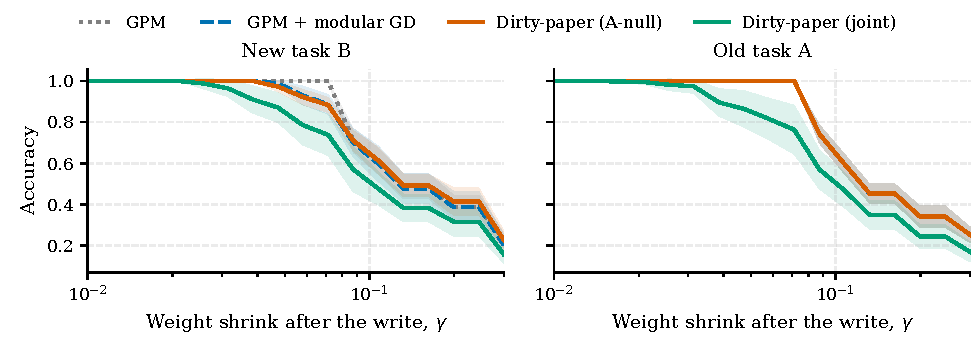
\includegraphics[width=\textwidth]{decay.pdf}
  \caption{\textbf{The joint write's old outputs are the first to fail under later training.}
  Accuracy after an exact write followed by a uniform weight shrink \(w\mapsto(1-\gamma)w\), at the main configuration.
  The A-null arms coincide on the old task; the joint arm, which moved old outputs by whole periods, loses them at smaller \(\gamma\).
  Means over \nseeds{} seeds with 95\% Student-\(t\) bands.}
  \label{fig:decay}
\end{figure}

\end{document}
